% -*-latex-*-
%
%  The contents of this file are subject to the University of Utah Public
%  License (the "License"); you may not use this file except in compliance
%  with the License.
%
%  Software distributed under the License is distributed on an "AS IS"
%  basis, WITHOUT WARRANTY OF ANY KIND, either express or implied. See the
%  License for the specific language governing rights and limitations under
%  the License.
%
%  The Original Source Code is SCIRun, released March 12, 2001.
%
%  The Original Source Code was developed by the University of Utah.
%  Portions created by UNIVERSITY are Copyright (C) 2001, 1994
%  University of Utah. All Rights Reserved.
%

% running.tex
%
% This is the `Running SCIRun' main section.

\chapter{Starting \sr{}}
\label{ch:startingup}


\section{Preparation}
\label{sec:prepare}

Preparations must be made before starting \sr{} and its Power Apps.
Commands below are typed in a terminal emulation application (\eg{}
\command{xterm}).

Create an ``on the fly libs'' directory and a \sr{}
initialization file:

\begin{alltt}
  mkdir ~/on-the-fly-libs
  echo "SCIRUN_ON_THE_FLY_LIBS_DIR=~/on-the-fly-libs" \latexhtml{\ra\ra}{\begin{rawhtml}&gt;&gt;\end{rawhtml}} .scirunrc
\end{alltt}

See \secref{Environment Variables}{sec:environ}, \secref{\sr{}'s
Initialization File---\filename{.scirunrc}}{sec:scirunrc},  and \secref{Dynamic
Compilation}{sec:dyncomp} for more information on \sr{}'s
environment variables, initialization file, and ``on the fly libs.''
  
Mac OSX users must increase the open files limit.
Users of csh-type shells on Mac OSX must type:

\begin{alltt}
  limit descriptors unlimited
\end{alltt}

and users of sh-type shells must type:

\begin{alltt}
  ulimit -n unlimited
\end{alltt}

%begin{latexonly}
\newcommand{\srwindow}%
{\centerline{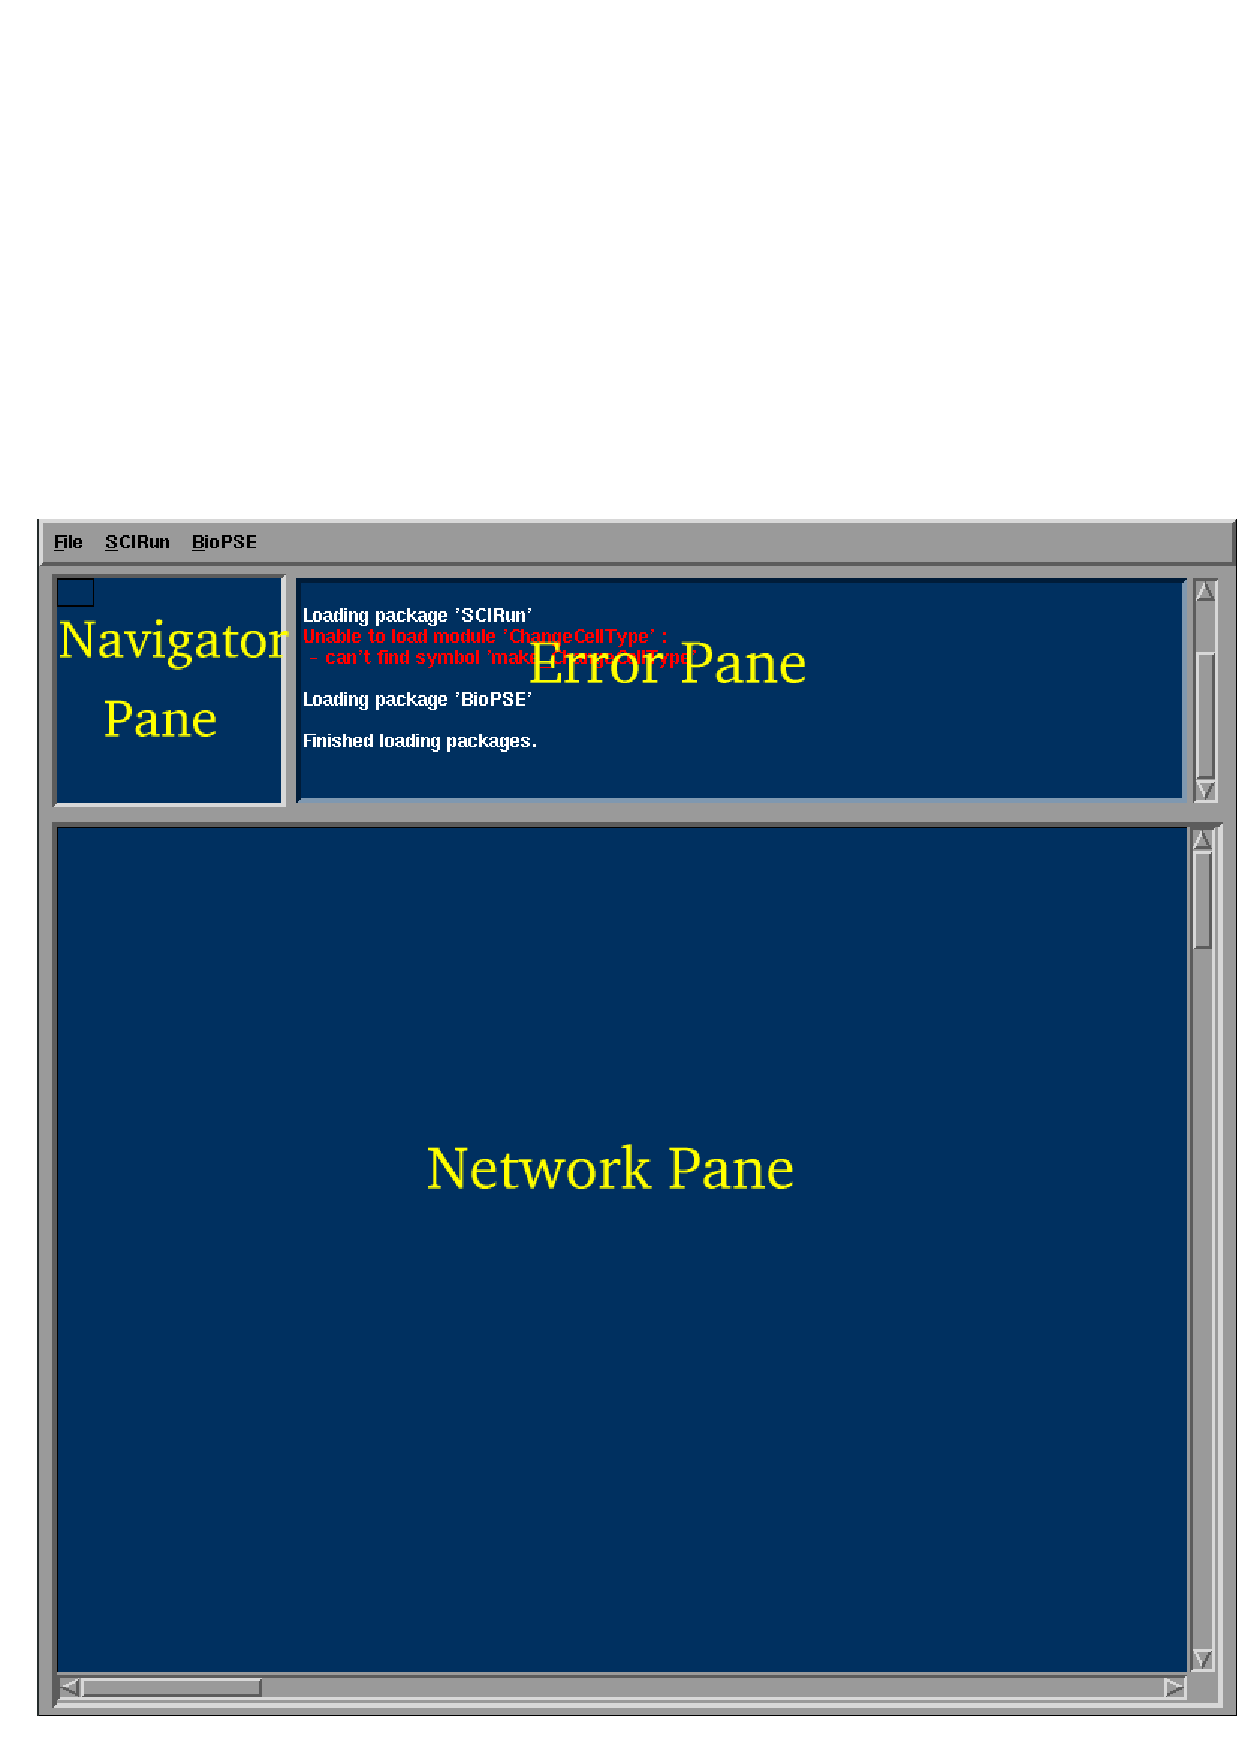
\epsfig{file=Figures/srwindow-1.eps.gz, width=6in,
      bbllx=0, bblly=0, bburx=400, bbury=410}}}
%end{latexonly}
\begin{htmlonly}
  \newcommand{\srwindow}{%
    \htmladdimg[align=top,alt="SCIRun Window"]
    {../Figures/srwindow-1.gif}}
\end{htmlonly}

Change your current working directory to \sr{}'s
build directory (for an installation from source code) or to
\filename{/usr/local/SCIRun/bin} (for an installation from an RPM):

\begin{alltt}
  cd SCIRun/sgi32
\end{alltt}

or

\begin{alltt}
  cd /usr/local/SCIRun/bin
\end{alltt}

and type:

\begin{alltt}
  ./scirun \replaceable{network_file}
\end{alltt}

\note{Do not start \sr{} in the background, \ie do not type
  \keyboard{scirun~\&}.}

The \command{scirun} command may take 1 argument, the name of a
\dfn{\sr{} network file} (network files have a \filename{.net} extension)
for \sr{} to load.  Network files are discussed in a later section.

If the name of a network file is not provided, \sr{} starts with a
blank window as shown in Figure~\ref{fig:srwindow}.  \secref{Anatomy
  of the Main Window}{sec:windowanatomy} discusses the main features
of Main Window window.

\begin{figure}[htb]
  \begin{makeimage}
  \end{makeimage}
  \srwindow
  \caption{\label{fig:srwindow} \sr{} Main Window}
\end{figure}

\sr{} may encounter errors during start up.  Errors, warnings, and
other messages are displayed in \sr{}'s error frame (see
Figure~\ref{fig:srwindow}).  Errors should be
\htmladdnormallink{reported}{\bugsurl} to the \sr{} development team
(See \secref{Reporting Bugs}{sec:bugs} for information on reporting
bugs).

\section{Anatomy of the Main Window}
\label{sec:windowanatomy}

The \sr{} main window consists of the Menu Bar, the Global View Frame,
the Error Frame, and the NetEdit frame (see
Figure~\ref{fig:srwindow}):

\begin{description}
  \descitem{Menu Bar} The menu bar is used to load networks, save
  networks, quit \sr{}, create network modules, and perform other
  tasks.  The menu bar consists of the following menu items:

  \begin{description}
    \menudesc{File} The \menu{File} menu contains the following items:

    \begin{description}
      \menuitemdesc{Save} Saves a network to a file (See \hyperref{this
        section}{Section~}{}{sec:savenet}).

      \menuitemdesc{Save As...} Saves a network to a new file (See
      \hyperref{this section}{Section~}{}{sec:savenet}).
      
      \menuitemdesc{Load} Loads a network from a file (See
      \hyperref{this section}{Section~}{}{sec:opennet}).
      
      \menuitemdesc{Insert} Adds a network to the NetEdit frame
      without overlap (See \hyperref{this
        section}{Section~}{}{sec:insertnetwork}).
      
      \menuitemdesc{Clear} Removes all modules and connections from
      the NetEdit frame (See \hyperref{this
        section}{Section~}{}{sec:clearnetwork}).
      
      \menuitemdesc{New} Contains items of interest to
      developers only.
      
      \menuitemdesc{Add Info} Adds network specific
      notes to the current network.  Notes should be used to document
      the purpose of the network (See \hyperref{this
        section}{Section~}{}{sec:docnetwork}).
    
      \menuitemdesc{Quit} Quits \sr{}
    \end{description}
  \end{description}
  
  \begin{description}
    \menudesc{SCIRun} The \menu{SCIRun} menu is used to create modules
    (from the \sr{} package) for use in the net edit frame.

    This menu is composed of sub-menus. Each sub-menu corresponds to
     a \dfn{category}
    \index{category} within the \sr{} package.  A category is a group of
    related modules.  Each menu item in a category sub-menu creates a
    specific module and places it in the NetEdit frame.  
    
    The NetEdit frame pop-up menu  also
    provides access to the \menu{\sr{}} and \menu{\biopse{}} (and
    possibly other) package menus. Activate the NetEdit frame pop-up
    menu by clicking Btn3 (right mouse button). \secref{The
      \biopse{}Package}{sec:biopsepackage} has an overview of the
    \sr{} package.
  \end{description}

  \begin{description}
    \menudesc{BioPSE} The \menu{BioPSE} menu creates modules (from the
    \biopse package) for use in the NetEdit frame.  It consists of
    category sub-menus and module menu items \secref{The SCIRun
      Package}{sec:srpackage} has an overview of the \biopse{}package.
  \end{description}

  \begin{description}
    \descitem{\ptext{Other Package Menus}} There may be other
    package menus if other packages have been installed.  They also
    have category sub-menus and module menu items.
  \end{description}
  
  \descitem{Global View Frame} The Global View Frame is located in the
  upper left corner of the main window (see
  Figure~\ref{fig:srwindow}). It is used to navigate complex networks
  \secref{Navigating a Network}{sec:navnetwork} describes the use of the Global View Frame.
  
  \descitem{Error Frame} Errors during program startup are displayed
  in the Error Frame.  The Error Frame is located in the upper right
  corner of the main window (see Figure~\ref{fig:srwindow}).  Errors on
  startup may mean \sr{} has been installed incorrectly or has
  been installed from a buggy distribution.  Please report these
  errors (\hyperref{report}{see Section~}{)}{sec:bugs}).
  
  \descitem{NetEdit Frame} The NetEdit Frame occupies the bottom of
  the main window(see Figure~\ref{fig:srwindow}).  It is used to build
  and execute networks (\secref{Working with  Networks}{ch:workwithnets}
  discusses the use of the NetEdit frame).

\end{description}

\section{The Terminal Window}
\label{sec:termwinapp}

After starting, \sr{} runs a shell-like application in the
terminal window called the \dfn{\sr{} shell}.  The \sr{} shell displays the
prompt \screen{scirun\ra}.  This program is  a modified \dfna{Tool
  Command Language}{TCL} shell program. It is possible to type
\acronym{TCL}'ish \sr{} commands at the prompt.  \hyperref{A later
  section}{Section~}{}{sec:termapp} describes use of the SCIRun shell.


\section{Environment Variables}
\label{sec:environ} 
\index{Environment Variables}

\newcommand{\envitem}[1]{\item[\envvar{#1}]\latex{\mbox{}\\}}

The following environment variables affect \sr{}'s behavior, or
improve its performance via remote connections.  With the exception of
\envvar{SCIRUN\_ON\_THE\_FLY\_LIBS\_DIR}, use of these variables is
optional.

\begin{description}
  \envitem{SCIRUN\_ON\_THE\_FLY\_LIBS\_DIR}
  \envvar{SCIRUN\_ON\_THE\_FLY\_LIBS\_DIR} specifies the location of
  dynamically generated code (see \secref{Dynamic
  Compilation}{sec:dyncomp} for details on the meaning and use of
  this variable).  Typically, a user should create directory
  \directory{\ltilde{}/on\_the\_fly}, and then, in his login script or
  \filename{.scirunrc} file set the value of 
  \envvar{SCIRUN\_ON\_THE\_FLY\_LIBS\_DIR} to \directory{\ltilde{}/on\_the\_fly}.
  
  \envitem{SCI\_CONFIRM\_OVERWRITE} determines the default behavior of
  file saving operations.  If set to 1, the user is always
  asked to confirm a file save if an existing file would be
  overwritten.  If set to 0 then the user is not asked for
  confirmation.  If \envvar{SCI\_CONFIRM\_OVERWRITE} is undefined, a
  value of 1 is assumed.
  
  \descitem{\envvar{SCIRUN\_DATA},  \envvar{SCIRUN\_DATASET}} These
  two variables specify the complete path to a \sr{} \dfn{data set}. A
  data set is a collection of \sr{} type data fields, matrices, \etc{}
  that are stored in a directory and used in \sr{} networks.

  \envvar{SCIRUN\_DATA} specifies a directory that contains a
  collection of data set directories.  \envvar{SCIRUN\_DATA} is used in
  conjunction with \envvar{SCIRUN\_DATASET} to specify the full path of
  a data set.  \envvar{SCIRUN\_DATASET} specifies a specific data set
  directory. 

  When working with the sample \sr{} data sets, for example,
  \envvar{SCIRUN\_DATA} is set to
  \filename{/usr/local/SCIRunData} (assuming this is where \sr{}'s
  sample data were installed).  \envvar{SCIRUN\_DATASET} can then be
  set to \filename{utahtorso} to specify the Utah Torso data set.
  
  \envitem{DISPLAY} If \sr{} is executed remotely, the value of
  the \envvar{DISPLAY} variable (as set on the remote machine) must be
  set correctly, and the remote machine must be allowed to talk to the
  local X11 server.
  
  For telnet-like (unencrypted) connections to a remote machine,
 set \envvar{DISPLAY} as follows:

for a sh-style shell

\begin{verbatim}
  export DISPLAY=local-ip-addres:0.0
\end{verbatim}
  
for a csh-style shell

\begin{verbatim}
  setenv DISPLAY local-ip-addres:0.0
\end{verbatim}

  When connecting to a remote machine using ssh, \envvar{DISPLAY} is
  usually set automatically (depending on how ssh has been
  configured).  However, this results in poor display performance
  because of encryption activity on the connection.  To increase
  performance, override the value of \envvar{DISPLAY} provided
  by ssh by setting  \envvar{DISPLAY} as
  shown above.  Note that this technique defeats the encryption
  protection on the X11 connection.
  
  The remote machine needs permission to display on a local machine if
  the user is using a telnet-like connection, or overriding the value
  of \envvar{DISPLAY} provided by ssh.  Use the \command{xhost}
  command on the local machine to do this:

\begin{verbatim}
  xhost +remote-machine-name
\end{verbatim}
  
  \envitem{LOAD\_PACKAGE} A comma separated list of package names that
  \sr{} loads.
  
  \sr{} loads these packages instead of packages specified at
  configure time. Each package on the list must be previously
  compiled.
  
  \envitem{PACKAGE\_SRC\_PATH} A colon separated list of paths to
  package source trees.  The path
  \directory{\ptext{build\_dir}/Packages} is implicitly part of this
  list.  \ptext{build\_dir} is the directory where
  \command{configure} and \command{make} were run.
  
  \sr{} searches this path list to find XML description files and
  user interface code corresponding to packages
  specified in \envvar{LOAD\_PACKAGE}.
  
  Its value defaults to \directory{\ptext{build\_dir}/Packages}.
  
  \envitem{PACKAGE\_LIB\_PATH} \envvar{PACKAGE\_LIB\_PATH} is a colon
  separated list of paths to package libraries.
  
  \sr{} searches this path list to find package libraries
  that correspond to the packages specified in
  \envvar{LOAD\_PACKAGE}.
  
  Default value is \directory{\ptext{build\_dir}/lib}.

  
\end{description}

\section{\sr{}'s Initialization File---\filename{.scirunrc}}
\label{sec:scirunrc}

When \sr{} starts up, it looks for and
loads the content of the file \filename{.scirunrc}.  \sr{} searches for
\filename{.scirunrc} in this order:

\begin{enumerate}
\item Current working directory
\item Root of \sr's build directory
\item Home directory
\item Root of \sr's source code directory
\end{enumerate}

This file may contain assignment of values to variables and variable
substitution.

For example:

\begin{verbatim}
HOME=/home/sci/me
SCIRUN_ON_THE_FLY_LIBS_DIR=$(HOME)/on-the-fly-libs
\end{verbatim}

The expansion of environment variables is not supported.  Only
variables declared earlier in the file can be expanded.

The following variables are understood by \sr{} and may be set in
\filename{.scirunrc}: \envvar{SCIRUN\_ON\_THE\_FLY\_LIBS\_DIR},
\envvar{LOAD\_PACKAGE}, \envvar{PACKAGE\_SRC\_PATH},
\envvar{PACKAGE\_LIB\_PATH}

\secref{Dynamic Compilation}{sec:dyncomp} explains the meaning and use
of \envvar{SCIRUN\_ON\_THE\_FLY\_LIBS\_DIR}. (See \hyperref{the
  previous section}{Section~}{}{sec:environ} for meanings of other
variables).

\section{Dynamic Compilation}
\label{sec:dyncomp}

Before executing \sr{},  be aware of the
\dfn{Dynamic Compilation} feature.

Dynamic compilation is a technique used by \sr{} to discover and
generate code for data types and algorithms used by modules in
networks.  This is done at runtime and once for each new
data type and algorithm encountered.  This technique provides a number
of benefits not discussed here (see the publication 
\htmladdnormallinkfoot{\etitle{Dynamic
    Compilation of C++ Template Code}}{http://www.sci.utah.edu/publications/mcole01/dyn.pdf}
for details).

By default, code generated by dynamic compilation is stored in the
directory \directory{\ptext{build\_dir}/on-the-fly-libs} 
(\ptext{build\_dir} is the directory in which \sr{} was built).  The
location of dynamically generated code can be changed by setting the
value of the environment variable
\envvar{SCI\_ON\_THE\_FLY\_LIBS\_DIR} to the desired directory. 

For example:

for Bourne-like shells (sh, ksh, bash, etc,)

\begin{verbatim}
SCIRUN_ON_THE_FLY_LIBS_DIR=$HOME/on-the-fly-libs
export SCIRUN_ON_THE_FLY_LIBS_DIR
\end{verbatim}

for csh-like shells

\begin{verbatim}
setenv SCIRUN_ON_THE_FLY_LIBS_DIR $HOME/on-the-fly-libs
\end{verbatim}

SCIRUN\_ON\_THE\_FLY\_LIBS\_DIR can be set in the user's
\filename{.scirunrc} file.

\begin{verbatim}
SCIRUN_ON_THE_FLY_LIBS_DIR=/home/me/on-the-fly-libs
\end{verbatim}

Setting a unique value of SCIRUN\_ON\_THE\_FLY\_LIBS\_DIR for each
\sr{} user has the following benefits:

\begin{itemize}
\item Allows multiple users to run the same instance of \sr{} without worry of  dynamic compilation conflicts.
  For example, by specifying an \filename{on-the-fly-libs}
  directory in their home directory, a user can run 
  \sr{} installed in \directory{/usr/local} that another user
  is already running.

\item Allows a \directory{/usr/local} installation of \sr{}
  to be secure because it does not require
  \directory{/usr/local/.../on-the-fly-libs} to be writable by
  all (a potential security risk).

\item Allows greater debugging and multiple build support by
  allowing the user to change dynamically compiled code locations
  between instances of \sr{}.

\end{itemize}

Dynamic compilation causes a delay the first time a module is
executed.  The module changes color while it is being
compiled.

\section{Exiting \sr{}}
\label{sec:stopping}

Exit \sr{} by selecting the \menuitem{Quit} item from the \menu{File} menu

Do not press \keyboard{control-c} to exit \sr{}.  Doing this will drop
\sr{} into a debugger.


%%% Local Variables: 
%%% mode: latex
%%% TeX-master: "usersguide"
%%% End: 
